\subsection{Time and Space Analysis}
In this subsection, we evaluate both time and space improvements of each optimization on each query. We consider both before and after \emph{disk cache}. Moreover, the space improvement is considering the \textbf{total size} of the transferred tables between memory and disk. Execution time is measured in \emph{seconds}. \\

\begin{tabularx}{\textwidth}{|*{7}{Y|}}
\hline
\multirow{2}{*}{Query 1} 
  &\multicolumn{3}{c|}{Before Cache}&\multicolumn{3}{c|}{After Cache}\\
\cline{2-7}
  &Time &Time \% &Space \% &Time &Time \% &Space \% \\
\hline
Initial Query &16.78 &- &- &1.77 &- &- \\
\hline
Index Opt. &- &- &- &- &- &- \\
\hline
Query Opt. &10.87 &35\% &25\% &0.39 &78\% &25\% \\
\hline
Schema Opt. &8.8 &19\% &99.8\% &0.33 &18\% &99.8\% \\
\hline
Memory Opt. &7.8 &11\% &- &0.3 &9\% &- \\
\hline
\end{tabularx} \\

\begin{tabularx}{\textwidth}{|*{7}{Y|}}
\hline
\multirow{2}{*}{Query 2} 
  &\multicolumn{3}{c|}{Before Cache}&\multicolumn{3}{c|}{After Cache}\\
\cline{2-7}
  &Time &Time \% &Space \% &Time &Time \% &Space \% \\
\hline
Initial Query &1535 &- &- &1463 &- &- \\
\hline
Index Opt. &9.49 &99\% &- &0.78 &99.9\% &- \\
\hline
Query Opt. &7.75 &18\% &- &0.68 &13\% &- \\
\hline
Schema Opt. &6.8 &12\% &99.8\% &0.65 &4\% &99.8\% \\
\hline
Memory Opt. &5.77 &15\% &- &0.65 &0\% &- \\
\hline
\end{tabularx} \\

\begin{tabularx}{\textwidth}{|*{7}{Y|}}
\hline
\multirow{2}{*}{Query 3} 
  &\multicolumn{3}{c|}{Before Cache}&\multicolumn{3}{c|}{After Cache}\\
\cline{2-7}
  &Time &Time \% &Space \% &Time &Time \% &Space \% \\
\hline
Initial Query &0.36 &- &- &0.07 &- &- \\
\hline
Index Opt. &0.23 &36\% &- &0.01 &85.7\% &- \\
\hline
Query Opt. &0.19 &17\% &- &0.01 &0\% &- \\
\hline
Schema Opt. &0.14 &26\% &99.8\% &0 &100\% &99.8\% \\
\hline
Memory Opt. &0.12 &14\% &- &0 &0\% &- \\
\hline
\end{tabularx} \\

\begin{tabularx}{\textwidth}{|*{7}{Y|}}
\hline
\multirow{2}{*}{Query 4} 
  &\multicolumn{3}{c|}{Before Cache}&\multicolumn{3}{c|}{After Cache}\\
\cline{2-7}
  &Time &Time \% &Space \% &Time &Time \% &Space \% \\
\hline
Initial Query &10.41 &- &- &0.27 &- &- \\
\hline
Index Opt. &- &- &- &- &- &- \\
\hline
Query Opt. &- &- &- &- &- &- \\
\hline
Schema Opt. &6.37 &39\% &99.8\% &0.15 &44\% &99.8\% \\
\hline
Memory Opt. &6.01 &5.5\% &- &0.13 &13\% &- \\
\hline
\end{tabularx} \\

\begin{tabularx}{\textwidth}{|*{7}{Y|}}
\hline
\multirow{2}{*}{Query 5} 
  &\multicolumn{3}{c|}{Before Cache}&\multicolumn{3}{c|}{After Cache}\\
\cline{2-7}
  &Time &Time \% &Space \% &Time &Time \% &Space \% \\
\hline
Initial Query &6.14 &- &- &0.33 &- &- \\
\hline
Index Opt. &- &- &- &- &- &- \\
\hline
Query Opt. &4.39 &28.5\% &- &0.26 &21\% &- \\
\hline
Schema Opt. &2.94 &33\% &99.85\% &0.21 &19\% &99.85\% \\
\hline
Memory Opt. &2.34 &20\% &- &0.2 &4.7\% &- \\
\hline
\end{tabularx} \\

\subsection{Database Size Effect}
The following plots show the effect of increasing database sizes on the execution time of our $5$ queries. We consider both before and after \emph{disk cache}.

\begin{figure}[H]
    \centering
    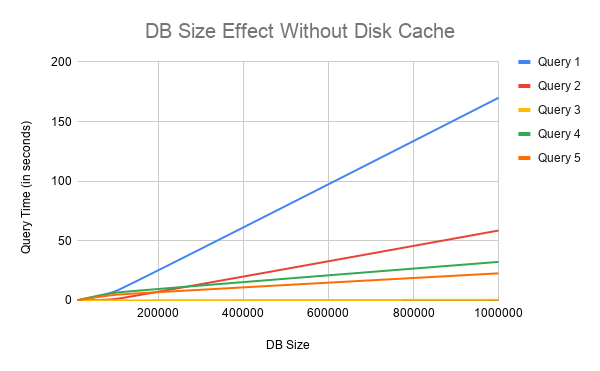
\includegraphics[width=0.8\textwidth]{images/db-size-without-cache.png}
    \caption{Database Size Effect Without OS (Disk) Cache.}
    \label{fig:db-size-1}
\end{figure}

\begin{figure}[H]
    \centering
    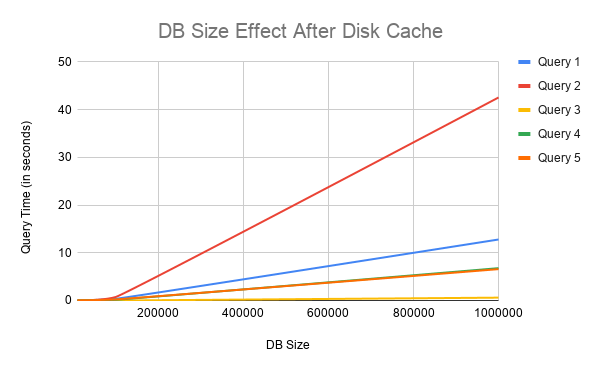
\includegraphics[width=0.8\textwidth]{images/db-size-after-cache .png}
    \caption{Database Size Effect After OS (Disk) Cache.}
    \label{fig:db-size-2}
\end{figure}

\subsection{Optimized SQL vs. NoSQL}

\subsection{Hardware Effect}
